\documentclass[a4paper, 10pt, twoside]{article}
\usepackage[left=2cm, right=2cm, top=2cm, bottom=3cm]{geometry}
\usepackage[super]{natbib}
\usepackage{amsmath}
\usepackage[shortlabels]{enumitem}
\usepackage{bbold}
\usepackage{graphicx}
\usepackage{url}
\usepackage{hyperref}
\hypersetup{
    colorlinks=true,
    linkcolor=blue,
    filecolor=magenta,      
    urlcolor=cyan,
}

\begin{document}

\title{High Performance Computing - Micro Aevol}
\author{T\'eo Bouvard}
\maketitle

\section{Introduction}
\section{Analyse}
\subsection{Version CPU}
Afin de se familiariser avec le code, il est intéressant de profiler son exécution. Cela permet d'identifier la structure globale du programme ainsi que son chemin critique.
\begin{figure}
	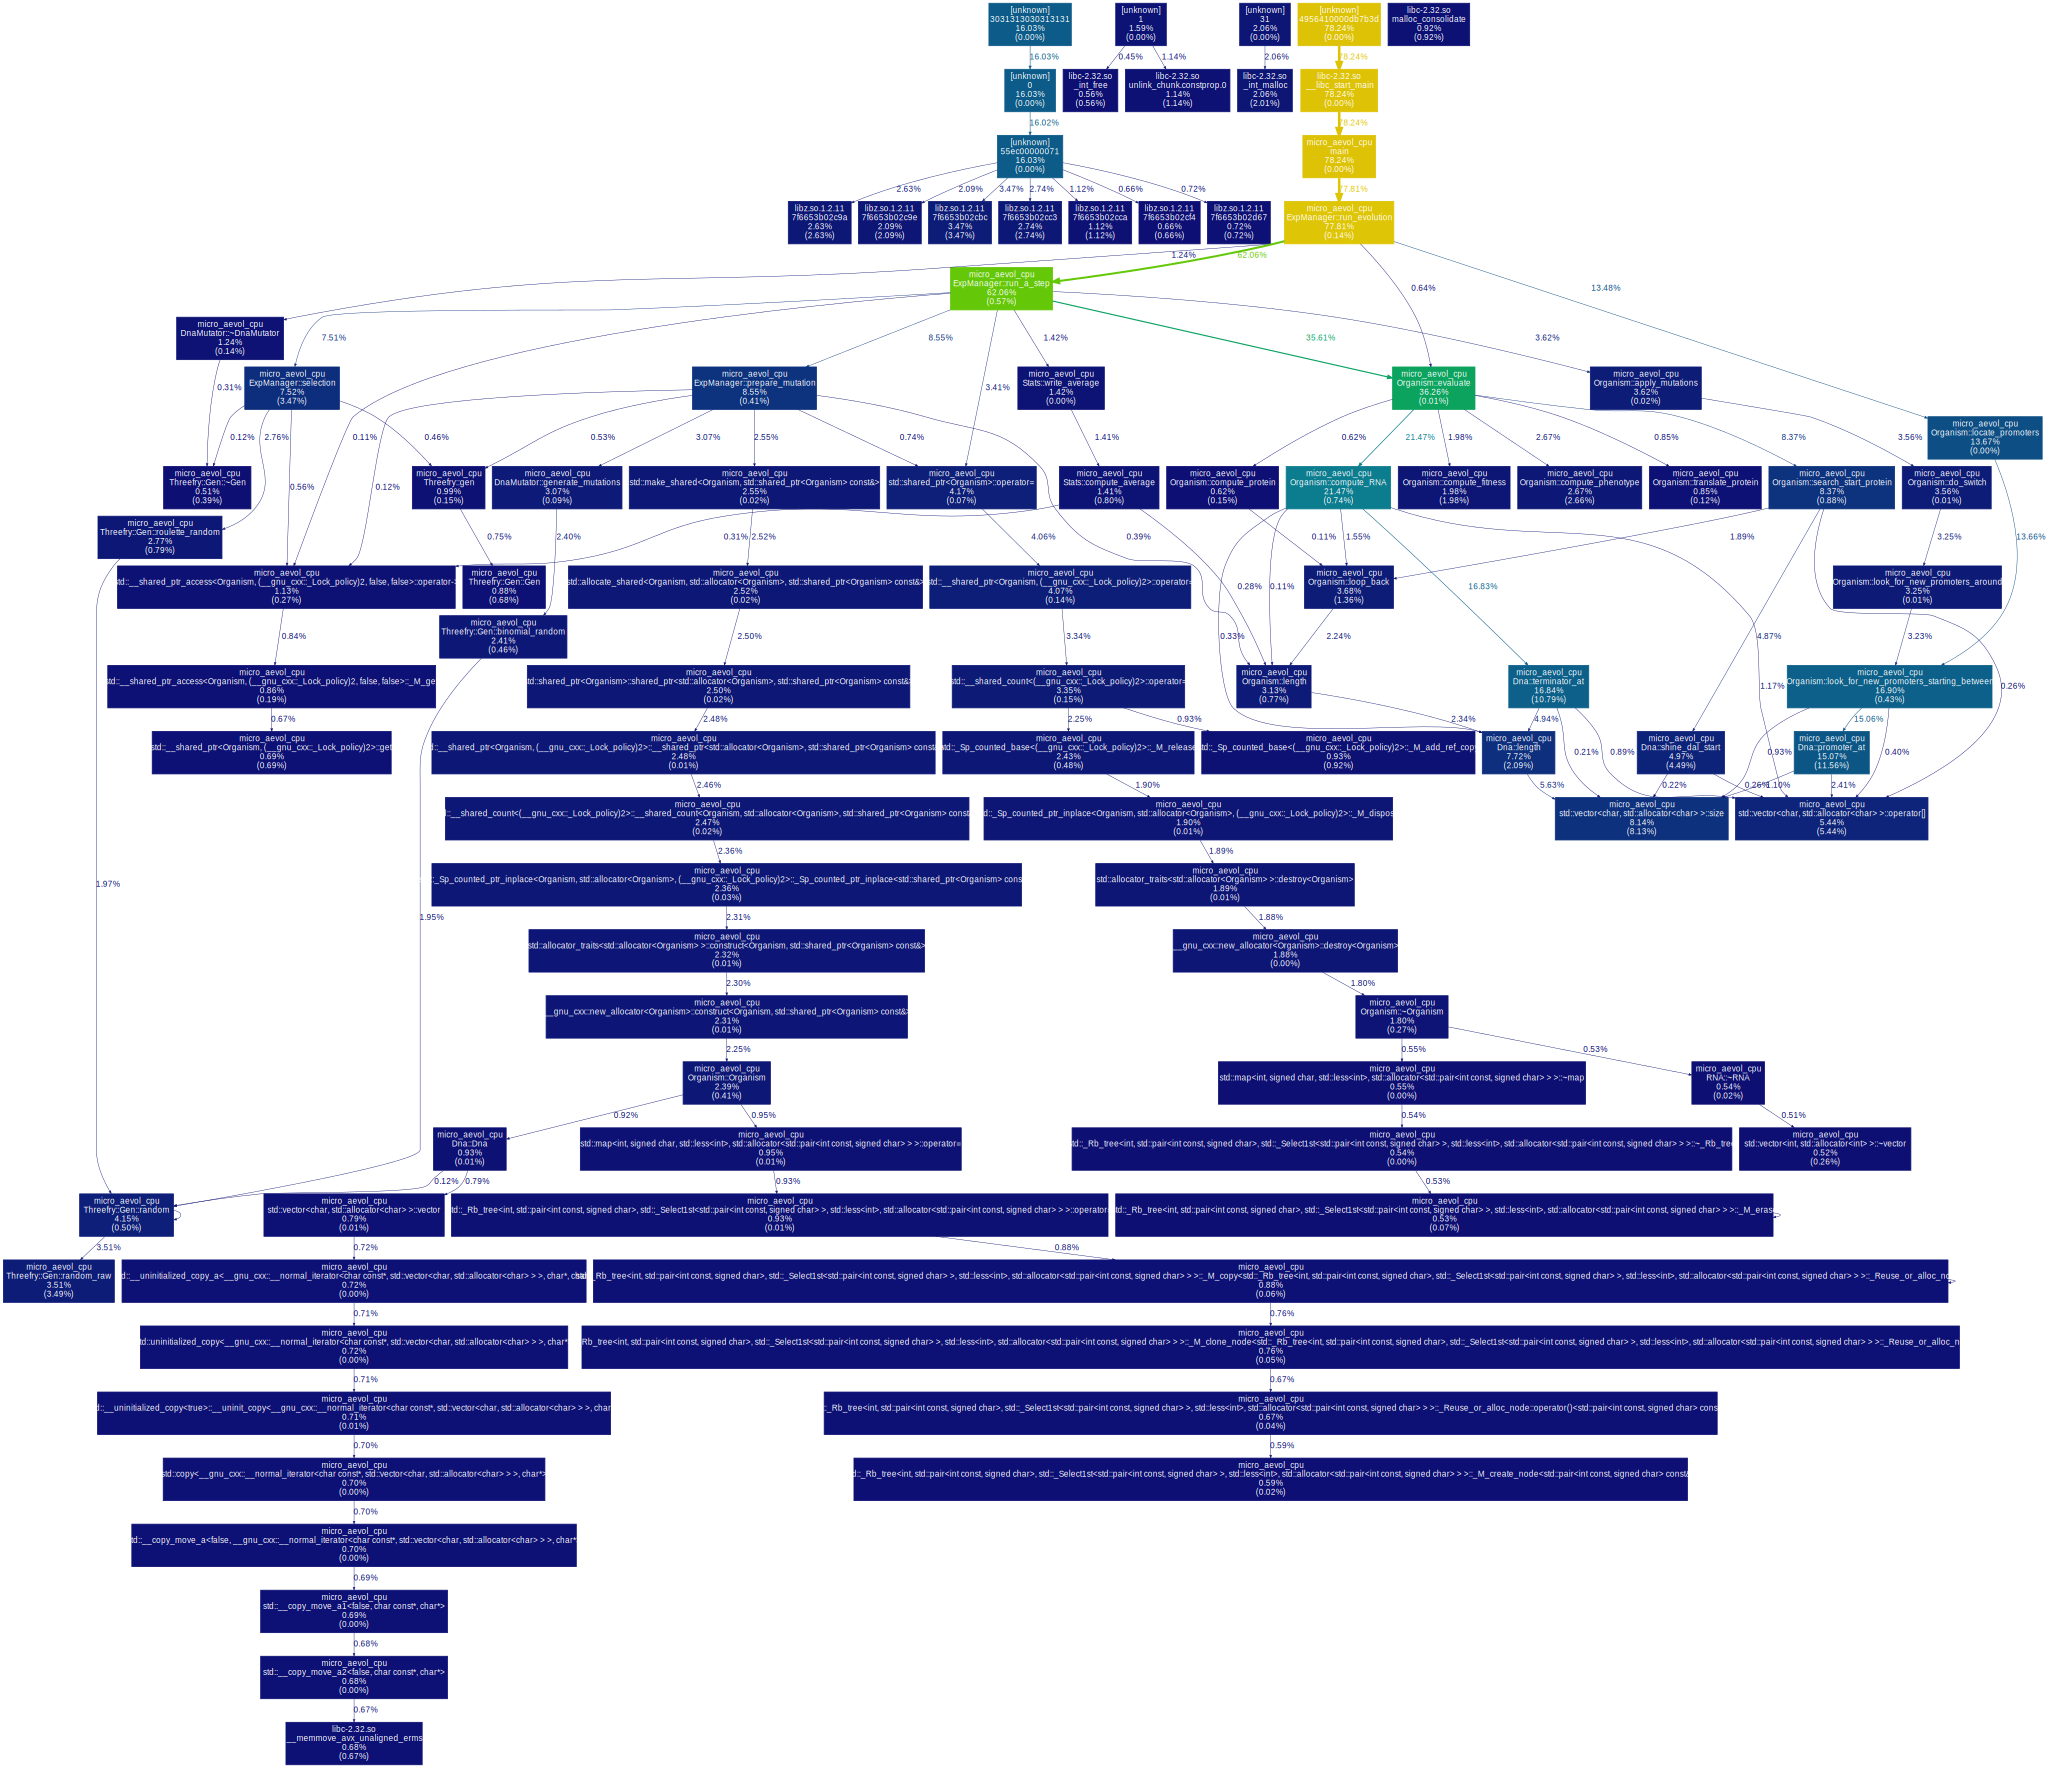
\includegraphics[width=\linewidth]{img/init_profile_debug.png}
\end{figure}
\subsection{Version GPU}

Divergence \citep{nvidia/branching}


\bibliographystyle{unsrtnat}
\bibliography{report}

\end{document}
